\documentclass[]{tufte-handout}

% ams
\usepackage{amssymb,amsmath}

\usepackage{ifxetex,ifluatex}
\usepackage{fixltx2e} % provides \textsubscript
\ifnum 0\ifxetex 1\fi\ifluatex 1\fi=0 % if pdftex
  \usepackage[T1]{fontenc}
  \usepackage[utf8]{inputenc}
\else % if luatex or xelatex
  \makeatletter
  \@ifpackageloaded{fontspec}{}{\usepackage{fontspec}}
  \makeatother
  \defaultfontfeatures{Ligatures=TeX,Scale=MatchLowercase}
  \makeatletter
  \@ifpackageloaded{soul}{
     \renewcommand\allcapsspacing[1]{{\addfontfeature{LetterSpace=15}#1}}
     \renewcommand\smallcapsspacing[1]{{\addfontfeature{LetterSpace=10}#1}}
   }{}
  \makeatother

\fi

% graphix
\usepackage{graphicx}
\setkeys{Gin}{width=\linewidth,totalheight=\textheight,keepaspectratio}

% booktabs
\usepackage{booktabs}

% url
\usepackage{url}

% hyperref
\usepackage{hyperref}

% units.
\usepackage{units}


\setcounter{secnumdepth}{-1}

% citations
\usepackage{natbib}
\bibliographystyle{plainnat}


% pandoc syntax highlighting
\usepackage{color}
\usepackage{fancyvrb}
\newcommand{\VerbBar}{|}
\newcommand{\VERB}{\Verb[commandchars=\\\{\}]}
\DefineVerbatimEnvironment{Highlighting}{Verbatim}{commandchars=\\\{\}}
% Add ',fontsize=\small' for more characters per line
\newenvironment{Shaded}{}{}
\newcommand{\AlertTok}[1]{\textcolor[rgb]{1.00,0.00,0.00}{\textbf{#1}}}
\newcommand{\AnnotationTok}[1]{\textcolor[rgb]{0.38,0.63,0.69}{\textbf{\textit{#1}}}}
\newcommand{\AttributeTok}[1]{\textcolor[rgb]{0.49,0.56,0.16}{#1}}
\newcommand{\BaseNTok}[1]{\textcolor[rgb]{0.25,0.63,0.44}{#1}}
\newcommand{\BuiltInTok}[1]{\textcolor[rgb]{0.00,0.50,0.00}{#1}}
\newcommand{\CharTok}[1]{\textcolor[rgb]{0.25,0.44,0.63}{#1}}
\newcommand{\CommentTok}[1]{\textcolor[rgb]{0.38,0.63,0.69}{\textit{#1}}}
\newcommand{\CommentVarTok}[1]{\textcolor[rgb]{0.38,0.63,0.69}{\textbf{\textit{#1}}}}
\newcommand{\ConstantTok}[1]{\textcolor[rgb]{0.53,0.00,0.00}{#1}}
\newcommand{\ControlFlowTok}[1]{\textcolor[rgb]{0.00,0.44,0.13}{\textbf{#1}}}
\newcommand{\DataTypeTok}[1]{\textcolor[rgb]{0.56,0.13,0.00}{#1}}
\newcommand{\DecValTok}[1]{\textcolor[rgb]{0.25,0.63,0.44}{#1}}
\newcommand{\DocumentationTok}[1]{\textcolor[rgb]{0.73,0.13,0.13}{\textit{#1}}}
\newcommand{\ErrorTok}[1]{\textcolor[rgb]{1.00,0.00,0.00}{\textbf{#1}}}
\newcommand{\ExtensionTok}[1]{#1}
\newcommand{\FloatTok}[1]{\textcolor[rgb]{0.25,0.63,0.44}{#1}}
\newcommand{\FunctionTok}[1]{\textcolor[rgb]{0.02,0.16,0.49}{#1}}
\newcommand{\ImportTok}[1]{\textcolor[rgb]{0.00,0.50,0.00}{\textbf{#1}}}
\newcommand{\InformationTok}[1]{\textcolor[rgb]{0.38,0.63,0.69}{\textbf{\textit{#1}}}}
\newcommand{\KeywordTok}[1]{\textcolor[rgb]{0.00,0.44,0.13}{\textbf{#1}}}
\newcommand{\NormalTok}[1]{#1}
\newcommand{\OperatorTok}[1]{\textcolor[rgb]{0.40,0.40,0.40}{#1}}
\newcommand{\OtherTok}[1]{\textcolor[rgb]{0.00,0.44,0.13}{#1}}
\newcommand{\PreprocessorTok}[1]{\textcolor[rgb]{0.74,0.48,0.00}{#1}}
\newcommand{\RegionMarkerTok}[1]{#1}
\newcommand{\SpecialCharTok}[1]{\textcolor[rgb]{0.25,0.44,0.63}{#1}}
\newcommand{\SpecialStringTok}[1]{\textcolor[rgb]{0.73,0.40,0.53}{#1}}
\newcommand{\StringTok}[1]{\textcolor[rgb]{0.25,0.44,0.63}{#1}}
\newcommand{\VariableTok}[1]{\textcolor[rgb]{0.10,0.09,0.49}{#1}}
\newcommand{\VerbatimStringTok}[1]{\textcolor[rgb]{0.25,0.44,0.63}{#1}}
\newcommand{\WarningTok}[1]{\textcolor[rgb]{0.38,0.63,0.69}{\textbf{\textit{#1}}}}

% table with pandoc

% multiplecol
\usepackage{multicol}

% strikeout
\usepackage[normalem]{ulem}

% morefloats
\usepackage{morefloats}


% tightlist macro required by pandoc >= 1.14
\providecommand{\tightlist}{%
  \setlength{\itemsep}{0pt}\setlength{\parskip}{0pt}}

% title / author / date
\title[Una Newsletter sull'andamento delle crypto]{Crypto News!}
\author{Enrico Pirani Max}
\date{}


\begin{document}

\maketitle




\hypertarget{importazione-delle-librerie-necessarie}{%
\subsection{Importazione delle librerie
necessarie}\label{importazione-delle-librerie-necessarie}}

In primo luogo, per eseguire il nostro processo di creazione di
strategie di trading, dobbiamo importare le librerie necessarie nel
nostro ambiente. In tutto questo processo, utilizzeremo alcune delle
librerie finanziarie più popolari in R, ovvero Quantmod, TTR e
Performance Analytics. Utilizzando la funzione library in R, possiamo
importare i nostri pacchetti richiesti.

\begin{Shaded}
\begin{Highlighting}[]
\NormalTok{y }\OtherTok{\textless{}{-}} \FunctionTok{rnorm}\NormalTok{(}\DecValTok{100}\NormalTok{)}
\NormalTok{x }\OtherTok{\textless{}{-}} \FunctionTok{rnorm}\NormalTok{(}\DecValTok{100}\NormalTok{)}
\NormalTok{m }\OtherTok{\textless{}{-}} \FunctionTok{lm}\NormalTok{(y }\SpecialCharTok{\textasciitilde{}}\NormalTok{ x)}
\FunctionTok{summary}\NormalTok{(x)}
\end{Highlighting}
\end{Shaded}

\begin{verbatim}
##     Min.  1st Qu.   Median     Mean  3rd Qu.     Max. 
## -2.38371 -0.77224 -0.09866 -0.07162  0.62338  2.08500
\end{verbatim}

\begin{Shaded}
\begin{Highlighting}[]
\FunctionTok{summary}\NormalTok{(m)}
\end{Highlighting}
\end{Shaded}

\begin{verbatim}
## 
## Call:
## lm(formula = y ~ x)
## 
## Residuals:
##     Min      1Q  Median      3Q     Max 
## -2.6502 -0.6489 -0.1231  0.6832  2.5922 
## 
## Coefficients:
##             Estimate Std. Error t value Pr(>|t|)
## (Intercept)  0.12643    0.10198   1.240    0.218
## x           -0.09846    0.10675  -0.922    0.359
## 
## Residual standard error: 1.017 on 98 degrees of freedom
## Multiple R-squared:  0.008607,   Adjusted R-squared:  -0.001509 
## F-statistic: 0.8508 on 1 and 98 DF,  p-value: 0.3586
\end{verbatim}

\begin{Shaded}
\begin{Highlighting}[]
\FunctionTok{library}\NormalTok{(quantmod)}
\end{Highlighting}
\end{Shaded}

\begin{verbatim}
## Loading required package: xts
\end{verbatim}

\begin{verbatim}
## Loading required package: zoo
\end{verbatim}

\begin{verbatim}
## 
## Attaching package: 'zoo'
\end{verbatim}

\begin{verbatim}
## The following objects are masked from 'package:base':
## 
##     as.Date, as.Date.numeric
\end{verbatim}

\begin{verbatim}
## Loading required package: TTR
\end{verbatim}

\begin{verbatim}
## Registered S3 method overwritten by 'quantmod':
##   method            from
##   as.zoo.data.frame zoo
\end{verbatim}

\begin{Shaded}
\begin{Highlighting}[]
\FunctionTok{library}\NormalTok{(PerformanceAnalytics)}
\end{Highlighting}
\end{Shaded}

\begin{verbatim}
## 
## Attaching package: 'PerformanceAnalytics'
\end{verbatim}

\begin{verbatim}
## The following object is masked from 'package:graphics':
## 
##     legend
\end{verbatim}

\begin{Shaded}
\begin{Highlighting}[]
\FunctionTok{library}\NormalTok{(TTR)}
\end{Highlighting}
\end{Shaded}

\hypertarget{passaggio-2-estrazione-dei-dati-da-yahoo-e-plotting-di-base}{%
\subsection{Passaggio 2: Estrazione dei dati da Yahoo e Plotting di
base}\label{passaggio-2-estrazione-dei-dati-da-yahoo-e-plotting-di-base}}

furante tutto il nostro processo, lavoreremo con i dati del prezzo delle
cryptovalute Bitcoin, Ethereum, Binance, Cardano e XRP. Estraiamo i dati
di queste valute da Yahoo in R.

\begin{Shaded}
\begin{Highlighting}[]
\FunctionTok{getSymbols}\NormalTok{(}\StringTok{"BTC{-}USD"}\NormalTok{, }\AttributeTok{src =} \StringTok{"yahoo"}\NormalTok{, }\AttributeTok{from =} \StringTok{"2019{-}01{-}01"}\NormalTok{)}
\end{Highlighting}
\end{Shaded}

\begin{verbatim}
## [1] "BTC-USD"
\end{verbatim}

\begin{Shaded}
\begin{Highlighting}[]
\FunctionTok{getSymbols}\NormalTok{(}\StringTok{"ETH{-}USD"}\NormalTok{, }\AttributeTok{src =} \StringTok{"yahoo"}\NormalTok{, }\AttributeTok{from =} \StringTok{"2019{-}01{-}01"}\NormalTok{)}
\end{Highlighting}
\end{Shaded}

\begin{verbatim}
## [1] "ETH-USD"
\end{verbatim}

\begin{Shaded}
\begin{Highlighting}[]
\FunctionTok{getSymbols}\NormalTok{(}\StringTok{"BNB{-}USD"}\NormalTok{, }\AttributeTok{src =} \StringTok{"yahoo"}\NormalTok{, }\AttributeTok{from =} \StringTok{"2019{-}01{-}01"}\NormalTok{)}
\end{Highlighting}
\end{Shaded}

\begin{verbatim}
## [1] "BNB-USD"
\end{verbatim}

\begin{Shaded}
\begin{Highlighting}[]
\FunctionTok{getSymbols}\NormalTok{(}\StringTok{"ADA{-}USD"}\NormalTok{, }\AttributeTok{src =} \StringTok{"yahoo"}\NormalTok{, }\AttributeTok{from =} \StringTok{"2019{-}01{-}01"}\NormalTok{)}
\end{Highlighting}
\end{Shaded}

\begin{verbatim}
## [1] "ADA-USD"
\end{verbatim}

\begin{Shaded}
\begin{Highlighting}[]
\FunctionTok{getSymbols}\NormalTok{(}\StringTok{"XRP{-}USD"}\NormalTok{, }\AttributeTok{src =} \StringTok{"yahoo"}\NormalTok{, }\AttributeTok{from =} \StringTok{"2019{-}01{-}01"}\NormalTok{)}
\end{Highlighting}
\end{Shaded}

\begin{verbatim}
## [1] "XRP-USD"
\end{verbatim}

\begin{Shaded}
\begin{Highlighting}[]
\FunctionTok{getSymbols}\NormalTok{(}\StringTok{"SOL{-}USD"}\NormalTok{, }\AttributeTok{src =} \StringTok{"yahoo"}\NormalTok{, }\AttributeTok{from =} \StringTok{"2020{-}01{-}01"}\NormalTok{)}
\end{Highlighting}
\end{Shaded}

\begin{verbatim}
## [1] "SOL-USD"
\end{verbatim}

Ora facciamo un po' di visualizzazione dei nostri dati estratti! Il
seguente codice produce un grafico a barre finanziario dei prezzi delle
azioni insieme al volume.

\begin{Shaded}
\begin{Highlighting}[]
\FunctionTok{barChart}\NormalTok{(}\StringTok{\textasciigrave{}}\AttributeTok{BTC{-}USD}\StringTok{\textasciigrave{}}\NormalTok{, }\AttributeTok{theme =} \FunctionTok{chartTheme}\NormalTok{(}\StringTok{"black"}\NormalTok{))}
\end{Highlighting}
\end{Shaded}

\includegraphics{cripto_update_files/figure-latex/unnamed-chunk-4-1}

\begin{Shaded}
\begin{Highlighting}[]
\FunctionTok{barChart}\NormalTok{(}\StringTok{\textasciigrave{}}\AttributeTok{BNB{-}USD}\StringTok{\textasciigrave{}}\NormalTok{, }\AttributeTok{theme =} \FunctionTok{chartTheme}\NormalTok{(}\StringTok{"black"}\NormalTok{))}
\end{Highlighting}
\end{Shaded}

\includegraphics{cripto_update_files/figure-latex/unnamed-chunk-4-2}

\begin{Shaded}
\begin{Highlighting}[]
\FunctionTok{barChart}\NormalTok{(}\StringTok{\textasciigrave{}}\AttributeTok{ETH{-}USD}\StringTok{\textasciigrave{}}\NormalTok{, }\AttributeTok{theme =} \FunctionTok{chartTheme}\NormalTok{(}\StringTok{"black"}\NormalTok{))}
\end{Highlighting}
\end{Shaded}

\includegraphics{cripto_update_files/figure-latex/unnamed-chunk-4-3}

\begin{Shaded}
\begin{Highlighting}[]
\FunctionTok{barChart}\NormalTok{(}\StringTok{\textasciigrave{}}\AttributeTok{ADA{-}USD}\StringTok{\textasciigrave{}}\NormalTok{, }\AttributeTok{theme =} \FunctionTok{chartTheme}\NormalTok{(}\StringTok{"black"}\NormalTok{))}
\end{Highlighting}
\end{Shaded}

\includegraphics{cripto_update_files/figure-latex/unnamed-chunk-4-4}

\begin{Shaded}
\begin{Highlighting}[]
\FunctionTok{barChart}\NormalTok{(}\StringTok{\textasciigrave{}}\AttributeTok{XRP{-}USD}\StringTok{\textasciigrave{}}\NormalTok{, }\AttributeTok{theme =} \FunctionTok{chartTheme}\NormalTok{(}\StringTok{"black"}\NormalTok{))}
\end{Highlighting}
\end{Shaded}

\includegraphics{cripto_update_files/figure-latex/unnamed-chunk-4-5}

\begin{Shaded}
\begin{Highlighting}[]
\FunctionTok{barChart}\NormalTok{(}\StringTok{\textasciigrave{}}\AttributeTok{SOL{-}USD}\StringTok{\textasciigrave{}}\NormalTok{, }\AttributeTok{theme =} \FunctionTok{chartTheme}\NormalTok{(}\StringTok{"black"}\NormalTok{))}
\end{Highlighting}
\end{Shaded}

\includegraphics{cripto_update_files/figure-latex/unnamed-chunk-4-6}

\hypertarget{creazione-di-indicatori-tecnici}{%
\subsection{Creazione di indicatori
tecnici}\label{creazione-di-indicatori-tecnici}}

Ci sono molti indicatori tecnici utilizzati per l'analisi finanziaria
ma, per la nostra analisi, utilizzeremo e creeremo sei dei più famosi
indicatori tecnici, ovvero: Media mobile semplice (SMA), Parabolic Stop
And Reverse (SAR), Indice del canale delle materie prime (CCI), Tasso di
variazione (ROC), Indice del momento stocastico (SMI) e infine Williams
\%R. Facciamolo!. Nella nuova dimensione di questi

\hypertarget{media-mobile-semplice-sma}{%
\subsubsection{Media mobile semplice
(SMA):}\label{media-mobile-semplice-sma}}

L'intervallo di tempo standard che prenderemo è di 20 giorni SMA e 50
giorni SMA. Ma non ci sono restrizioni nell'uso di qualsiasi intervallo
di tempo.

Il seguente codice calcolerà la SMA di tre aziende per 20 giorni e 50
giorni insieme ad un grafico:

\begin{Shaded}
\begin{Highlighting}[]
\NormalTok{BTC }\OtherTok{\textless{}{-}} \StringTok{\textasciigrave{}}\AttributeTok{BTC{-}USD}\StringTok{\textasciigrave{}}
\NormalTok{ETH }\OtherTok{\textless{}{-}} \StringTok{\textasciigrave{}}\AttributeTok{ETH{-}USD}\StringTok{\textasciigrave{}}
\NormalTok{BNB }\OtherTok{\textless{}{-}} \StringTok{\textasciigrave{}}\AttributeTok{BNB{-}USD}\StringTok{\textasciigrave{}}
\NormalTok{ADA }\OtherTok{\textless{}{-}} \StringTok{\textasciigrave{}}\AttributeTok{ADA{-}USD}\StringTok{\textasciigrave{}}
\NormalTok{XRP }\OtherTok{\textless{}{-}} \StringTok{\textasciigrave{}}\AttributeTok{XRP{-}USD}\StringTok{\textasciigrave{}}
\NormalTok{SOL }\OtherTok{\textless{}{-}} \StringTok{\textasciigrave{}}\AttributeTok{SOL{-}USD}\StringTok{\textasciigrave{}}
\end{Highlighting}
\end{Shaded}

\begin{Shaded}
\begin{Highlighting}[]
\CommentTok{\# 1. BTC{-}USD}
\NormalTok{sma50\_btc }\OtherTok{\textless{}{-}} \FunctionTok{SMA}\NormalTok{(BTC}\SpecialCharTok{$}\StringTok{\textasciigrave{}}\AttributeTok{BTC{-}USD.Close}\StringTok{\textasciigrave{}}\NormalTok{, }\AttributeTok{n =} \DecValTok{50}\NormalTok{)}
\NormalTok{sma100\_btc }\OtherTok{\textless{}{-}} \FunctionTok{SMA}\NormalTok{(BTC}\SpecialCharTok{$}\StringTok{\textasciigrave{}}\AttributeTok{BTC{-}USD.Close}\StringTok{\textasciigrave{}}\NormalTok{, }\AttributeTok{n =} \DecValTok{100}\NormalTok{)}
\FunctionTok{lineChart}\NormalTok{(}\StringTok{\textasciigrave{}}\AttributeTok{BTC{-}USD}\StringTok{\textasciigrave{}}\NormalTok{, }\AttributeTok{theme =} \FunctionTok{chartTheme}\NormalTok{(}\StringTok{"black"}\NormalTok{))}
\end{Highlighting}
\end{Shaded}

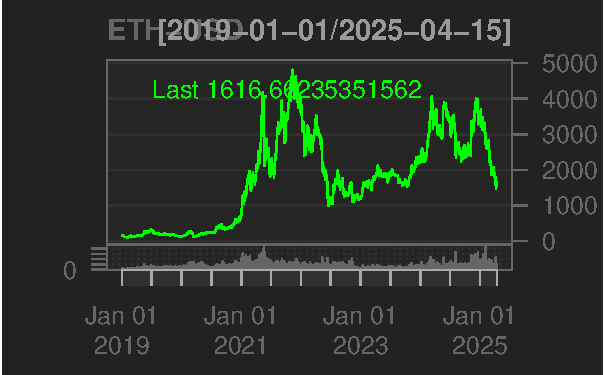
\includegraphics{cripto_update_files/figure-latex/unnamed-chunk-6-1}

\begin{Shaded}
\begin{Highlighting}[]
\FunctionTok{addSMA}\NormalTok{(}\AttributeTok{n =} \DecValTok{50}\NormalTok{, }\AttributeTok{col =} \StringTok{"blue"}\NormalTok{)}
\end{Highlighting}
\end{Shaded}

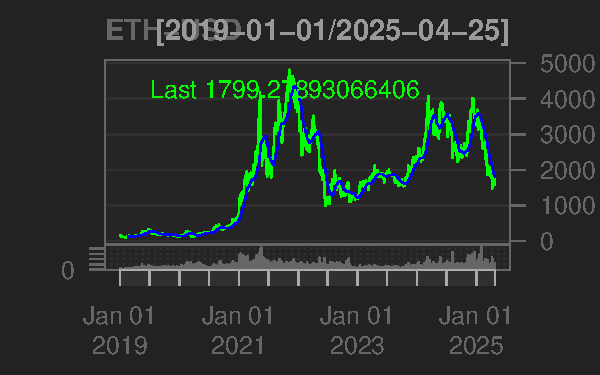
\includegraphics{cripto_update_files/figure-latex/unnamed-chunk-6-2}

\begin{Shaded}
\begin{Highlighting}[]
\FunctionTok{addSMA}\NormalTok{(}\AttributeTok{n =} \DecValTok{100}\NormalTok{, }\AttributeTok{col =} \StringTok{"orange"}\NormalTok{)}
\FunctionTok{legend}\NormalTok{(}\StringTok{"left"}\NormalTok{,}
  \AttributeTok{col =} \FunctionTok{c}\NormalTok{(}\StringTok{"green"}\NormalTok{, }\StringTok{"blue"}\NormalTok{, }\StringTok{"orange"}\NormalTok{),}
  \AttributeTok{legend =} \FunctionTok{c}\NormalTok{(}\StringTok{"BTC{-}USD"}\NormalTok{, }\StringTok{"SMA50"}\NormalTok{, }\StringTok{"SMA100"}\NormalTok{), }\AttributeTok{lty =} \DecValTok{1}\NormalTok{, }\AttributeTok{bty =} \StringTok{"n"}\NormalTok{,}
  \AttributeTok{text.col =} \StringTok{"white"}\NormalTok{, }\AttributeTok{cex =} \FloatTok{0.8}
\NormalTok{)}
\end{Highlighting}
\end{Shaded}

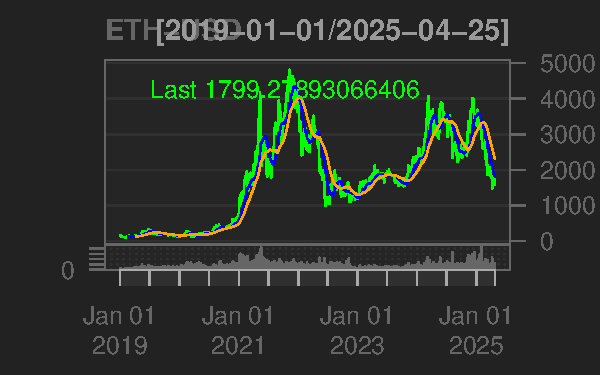
\includegraphics{cripto_update_files/figure-latex/unnamed-chunk-6-3}

\begin{Shaded}
\begin{Highlighting}[]
\CommentTok{\# 2. ETH{-}USD}
\NormalTok{sma50\_btc }\OtherTok{\textless{}{-}} \FunctionTok{SMA}\NormalTok{(ETH}\SpecialCharTok{$}\StringTok{\textasciigrave{}}\AttributeTok{ETH{-}USD.Close}\StringTok{\textasciigrave{}}\NormalTok{, }\AttributeTok{n =} \DecValTok{50}\NormalTok{)}
\NormalTok{sma100\_btc }\OtherTok{\textless{}{-}} \FunctionTok{SMA}\NormalTok{(ETH}\SpecialCharTok{$}\StringTok{\textasciigrave{}}\AttributeTok{ETH{-}USD.Close}\StringTok{\textasciigrave{}}\NormalTok{, }\AttributeTok{n =} \DecValTok{100}\NormalTok{)}
\FunctionTok{lineChart}\NormalTok{(}\StringTok{\textasciigrave{}}\AttributeTok{ETH{-}USD}\StringTok{\textasciigrave{}}\NormalTok{, }\AttributeTok{theme =} \FunctionTok{chartTheme}\NormalTok{(}\StringTok{"black"}\NormalTok{))}
\end{Highlighting}
\end{Shaded}

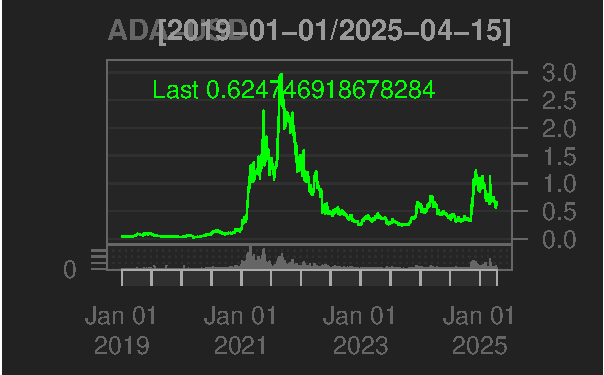
\includegraphics{cripto_update_files/figure-latex/unnamed-chunk-7-1}

\begin{Shaded}
\begin{Highlighting}[]
\FunctionTok{addSMA}\NormalTok{(}\AttributeTok{n =} \DecValTok{50}\NormalTok{, }\AttributeTok{col =} \StringTok{"blue"}\NormalTok{)}
\end{Highlighting}
\end{Shaded}

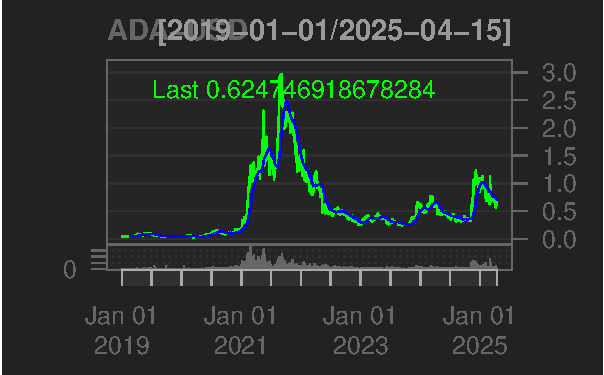
\includegraphics{cripto_update_files/figure-latex/unnamed-chunk-7-2}

\begin{Shaded}
\begin{Highlighting}[]
\FunctionTok{addSMA}\NormalTok{(}\AttributeTok{n =} \DecValTok{100}\NormalTok{, }\AttributeTok{col =} \StringTok{"orange"}\NormalTok{)}
\FunctionTok{legend}\NormalTok{(}\StringTok{"left"}\NormalTok{,}
  \AttributeTok{col =} \FunctionTok{c}\NormalTok{(}\StringTok{"green"}\NormalTok{, }\StringTok{"blue"}\NormalTok{, }\StringTok{"orange"}\NormalTok{),}
  \AttributeTok{legend =} \FunctionTok{c}\NormalTok{(}\StringTok{"ETH{-}USD"}\NormalTok{, }\StringTok{"SMA50"}\NormalTok{, }\StringTok{"SMA100"}\NormalTok{), }\AttributeTok{lty =} \DecValTok{1}\NormalTok{, }\AttributeTok{bty =} \StringTok{"n"}\NormalTok{,}
  \AttributeTok{text.col =} \StringTok{"white"}\NormalTok{, }\AttributeTok{cex =} \FloatTok{0.8}
\NormalTok{)}
\end{Highlighting}
\end{Shaded}

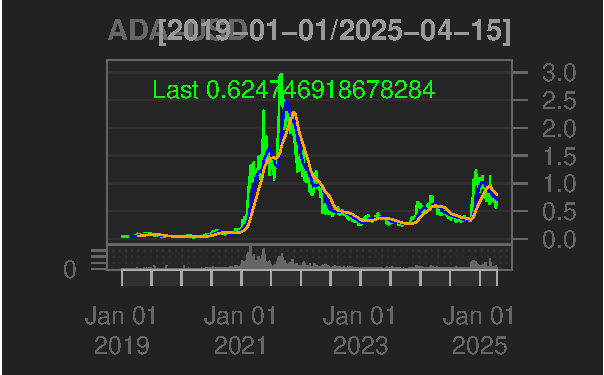
\includegraphics{cripto_update_files/figure-latex/unnamed-chunk-7-3}

\begin{Shaded}
\begin{Highlighting}[]
\NormalTok{sma50\_btc }\OtherTok{\textless{}{-}} \FunctionTok{SMA}\NormalTok{(ADA}\SpecialCharTok{$}\StringTok{\textasciigrave{}}\AttributeTok{ADA{-}USD.Close}\StringTok{\textasciigrave{}}\NormalTok{, }\AttributeTok{n =} \DecValTok{50}\NormalTok{)}
\NormalTok{sma100\_btc }\OtherTok{\textless{}{-}} \FunctionTok{SMA}\NormalTok{(ADA}\SpecialCharTok{$}\StringTok{\textasciigrave{}}\AttributeTok{ADA{-}USD.Close}\StringTok{\textasciigrave{}}\NormalTok{, }\AttributeTok{n =} \DecValTok{100}\NormalTok{)}
\FunctionTok{lineChart}\NormalTok{(}\StringTok{\textasciigrave{}}\AttributeTok{ADA{-}USD}\StringTok{\textasciigrave{}}\NormalTok{, }\AttributeTok{theme =} \FunctionTok{chartTheme}\NormalTok{(}\StringTok{"black"}\NormalTok{))}
\end{Highlighting}
\end{Shaded}

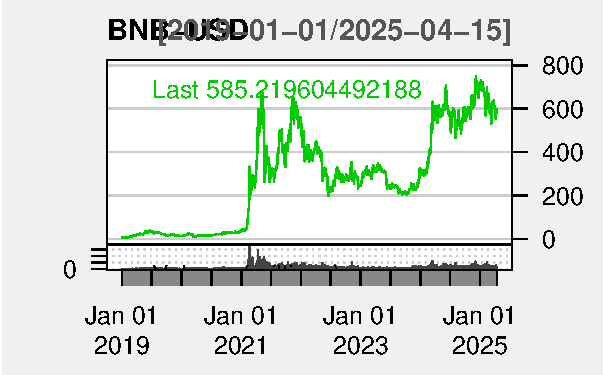
\includegraphics{cripto_update_files/figure-latex/unnamed-chunk-8-1}

\begin{Shaded}
\begin{Highlighting}[]
\FunctionTok{addSMA}\NormalTok{(}\AttributeTok{n =} \DecValTok{50}\NormalTok{, }\AttributeTok{col =} \StringTok{"blue"}\NormalTok{)}
\end{Highlighting}
\end{Shaded}

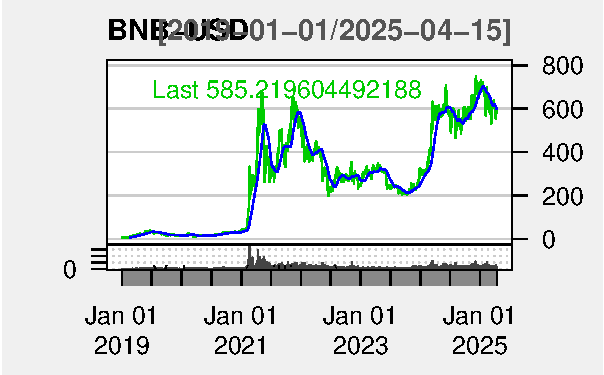
\includegraphics{cripto_update_files/figure-latex/unnamed-chunk-8-2}

\begin{Shaded}
\begin{Highlighting}[]
\FunctionTok{addSMA}\NormalTok{(}\AttributeTok{n =} \DecValTok{100}\NormalTok{, }\AttributeTok{col =} \StringTok{"orange"}\NormalTok{)}
\FunctionTok{legend}\NormalTok{(}\StringTok{"left"}\NormalTok{,}
  \AttributeTok{col =} \FunctionTok{c}\NormalTok{(}\StringTok{"green"}\NormalTok{, }\StringTok{"blue"}\NormalTok{, }\StringTok{"orange"}\NormalTok{),}
  \AttributeTok{legend =} \FunctionTok{c}\NormalTok{(}\StringTok{"ADA{-}USD"}\NormalTok{, }\StringTok{"SMA50"}\NormalTok{, }\StringTok{"SMA100"}\NormalTok{), }\AttributeTok{lty =} \DecValTok{1}\NormalTok{, }\AttributeTok{bty =} \StringTok{"n"}\NormalTok{,}
  \AttributeTok{text.col =} \StringTok{"white"}\NormalTok{, }\AttributeTok{cex =} \FloatTok{0.8}
\NormalTok{)}
\end{Highlighting}
\end{Shaded}

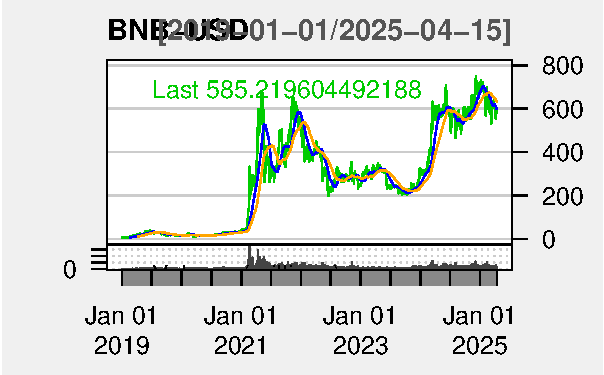
\includegraphics{cripto_update_files/figure-latex/unnamed-chunk-8-3}

\begin{Shaded}
\begin{Highlighting}[]
\NormalTok{sma50\_btc }\OtherTok{\textless{}{-}} \FunctionTok{SMA}\NormalTok{(BNB}\SpecialCharTok{$}\StringTok{\textasciigrave{}}\AttributeTok{BNB{-}USD.Close}\StringTok{\textasciigrave{}}\NormalTok{, }\AttributeTok{n =} \DecValTok{50}\NormalTok{)}
\NormalTok{sma100\_btc }\OtherTok{\textless{}{-}} \FunctionTok{SMA}\NormalTok{(BNB}\SpecialCharTok{$}\StringTok{\textasciigrave{}}\AttributeTok{BNB{-}USD.Close}\StringTok{\textasciigrave{}}\NormalTok{, }\AttributeTok{n =} \DecValTok{100}\NormalTok{)}
\FunctionTok{lineChart}\NormalTok{(}\StringTok{\textasciigrave{}}\AttributeTok{BNB{-}USD}\StringTok{\textasciigrave{}}\NormalTok{, }\AttributeTok{theme =} \FunctionTok{chartTheme}\NormalTok{(}\StringTok{"white"}\NormalTok{))}
\end{Highlighting}
\end{Shaded}

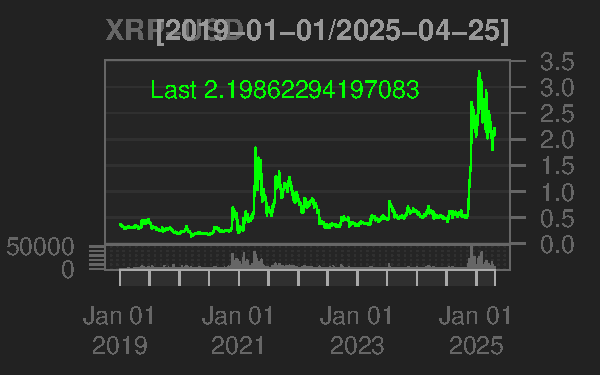
\includegraphics{cripto_update_files/figure-latex/unnamed-chunk-9-1}

\begin{Shaded}
\begin{Highlighting}[]
\FunctionTok{addSMA}\NormalTok{(}\AttributeTok{n =} \DecValTok{50}\NormalTok{, }\AttributeTok{col =} \StringTok{"blue"}\NormalTok{)}
\end{Highlighting}
\end{Shaded}

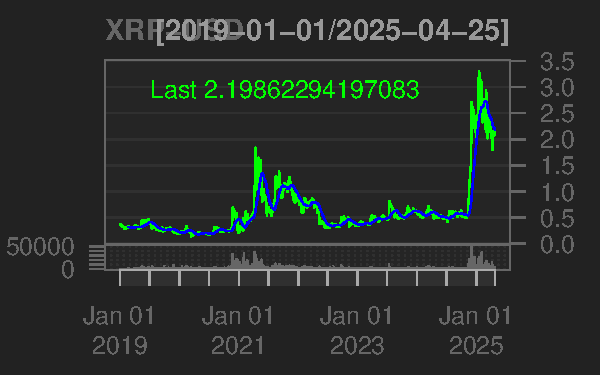
\includegraphics{cripto_update_files/figure-latex/unnamed-chunk-9-2}

\begin{Shaded}
\begin{Highlighting}[]
\FunctionTok{addSMA}\NormalTok{(}\AttributeTok{n =} \DecValTok{100}\NormalTok{, }\AttributeTok{col =} \StringTok{"orange"}\NormalTok{)}
\FunctionTok{legend}\NormalTok{(}\StringTok{"left"}\NormalTok{,}
  \AttributeTok{col =} \FunctionTok{c}\NormalTok{(}\StringTok{"green"}\NormalTok{, }\StringTok{"blue"}\NormalTok{, }\StringTok{"orange"}\NormalTok{),}
  \AttributeTok{legend =} \FunctionTok{c}\NormalTok{(}\StringTok{"BNB{-}USD"}\NormalTok{, }\StringTok{"SMA50"}\NormalTok{, }\StringTok{"SMA100"}\NormalTok{), }\AttributeTok{lty =} \DecValTok{1}\NormalTok{, }\AttributeTok{bty =} \StringTok{"n"}\NormalTok{,}
  \AttributeTok{text.col =} \StringTok{"white"}\NormalTok{, }\AttributeTok{cex =} \FloatTok{0.8}
\NormalTok{)}
\end{Highlighting}
\end{Shaded}

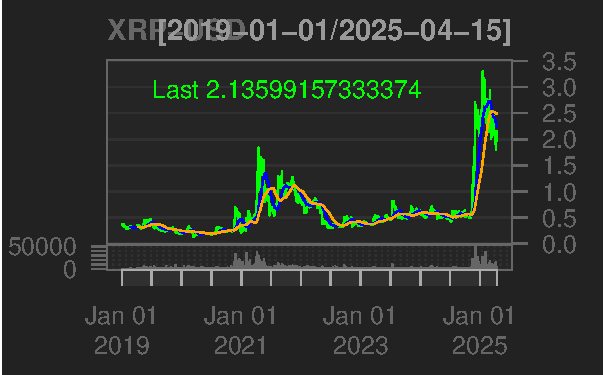
\includegraphics{cripto_update_files/figure-latex/unnamed-chunk-9-3}

\begin{Shaded}
\begin{Highlighting}[]
\NormalTok{sma50\_btc }\OtherTok{\textless{}{-}} \FunctionTok{SMA}\NormalTok{(XRP}\SpecialCharTok{$}\StringTok{\textasciigrave{}}\AttributeTok{XRP{-}USD.Close}\StringTok{\textasciigrave{}}\NormalTok{, }\AttributeTok{n =} \DecValTok{50}\NormalTok{)}
\NormalTok{sma100\_btc }\OtherTok{\textless{}{-}} \FunctionTok{SMA}\NormalTok{(XRP}\SpecialCharTok{$}\StringTok{\textasciigrave{}}\AttributeTok{XRP{-}USD.Close}\StringTok{\textasciigrave{}}\NormalTok{, }\AttributeTok{n =} \DecValTok{100}\NormalTok{)}
\FunctionTok{lineChart}\NormalTok{(}\StringTok{\textasciigrave{}}\AttributeTok{XRP{-}USD}\StringTok{\textasciigrave{}}\NormalTok{, }\AttributeTok{theme =} \FunctionTok{chartTheme}\NormalTok{(}\StringTok{"black"}\NormalTok{))}
\end{Highlighting}
\end{Shaded}

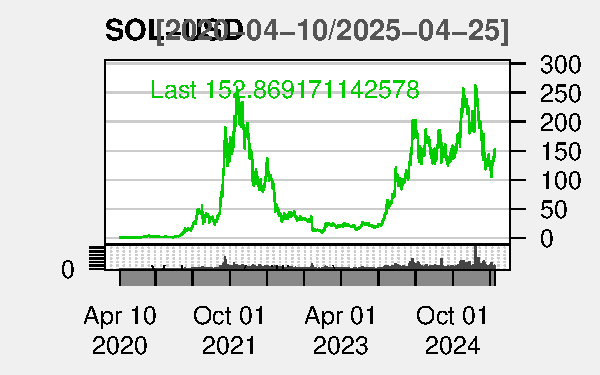
\includegraphics{cripto_update_files/figure-latex/unnamed-chunk-10-1}

\begin{Shaded}
\begin{Highlighting}[]
\FunctionTok{addSMA}\NormalTok{(}\AttributeTok{n =} \DecValTok{50}\NormalTok{, }\AttributeTok{col =} \StringTok{"blue"}\NormalTok{)}
\end{Highlighting}
\end{Shaded}

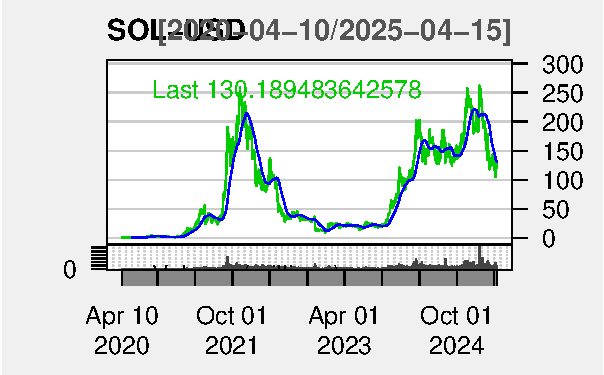
\includegraphics{cripto_update_files/figure-latex/unnamed-chunk-10-2}

\begin{Shaded}
\begin{Highlighting}[]
\FunctionTok{addSMA}\NormalTok{(}\AttributeTok{n =} \DecValTok{100}\NormalTok{, }\AttributeTok{col =} \StringTok{"orange"}\NormalTok{)}
\FunctionTok{legend}\NormalTok{(}\StringTok{"left"}\NormalTok{,}
  \AttributeTok{col =} \FunctionTok{c}\NormalTok{(}\StringTok{"green"}\NormalTok{, }\StringTok{"blue"}\NormalTok{, }\StringTok{"orange"}\NormalTok{),}
  \AttributeTok{legend =} \FunctionTok{c}\NormalTok{(}\StringTok{"BNB{-}USD"}\NormalTok{, }\StringTok{"SMA50"}\NormalTok{, }\StringTok{"SMA100"}\NormalTok{), }\AttributeTok{lty =} \DecValTok{1}\NormalTok{, }\AttributeTok{bty =} \StringTok{"n"}\NormalTok{,}
  \AttributeTok{text.col =} \StringTok{"white"}\NormalTok{, }\AttributeTok{cex =} \FloatTok{0.8}
\NormalTok{)}
\end{Highlighting}
\end{Shaded}

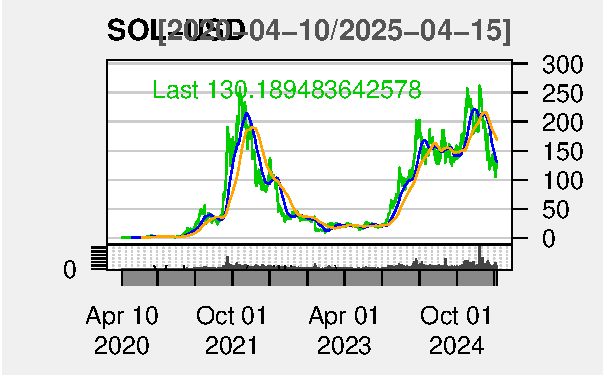
\includegraphics{cripto_update_files/figure-latex/unnamed-chunk-10-3}

\begin{Shaded}
\begin{Highlighting}[]
\NormalTok{sma50\_btc }\OtherTok{\textless{}{-}} \FunctionTok{SMA}\NormalTok{(SOL}\SpecialCharTok{$}\StringTok{\textasciigrave{}}\AttributeTok{SOL{-}USD.Close}\StringTok{\textasciigrave{}}\NormalTok{, }\AttributeTok{n =} \DecValTok{50}\NormalTok{)}
\NormalTok{sma100\_btc }\OtherTok{\textless{}{-}} \FunctionTok{SMA}\NormalTok{(SOL}\SpecialCharTok{$}\StringTok{\textasciigrave{}}\AttributeTok{SOL{-}USD.Close}\StringTok{\textasciigrave{}}\NormalTok{, }\AttributeTok{n =} \DecValTok{100}\NormalTok{)}
\FunctionTok{lineChart}\NormalTok{(}\StringTok{\textasciigrave{}}\AttributeTok{SOL{-}USD}\StringTok{\textasciigrave{}}\NormalTok{, }\AttributeTok{theme =} \FunctionTok{chartTheme}\NormalTok{(}\StringTok{"white"}\NormalTok{))}
\end{Highlighting}
\end{Shaded}

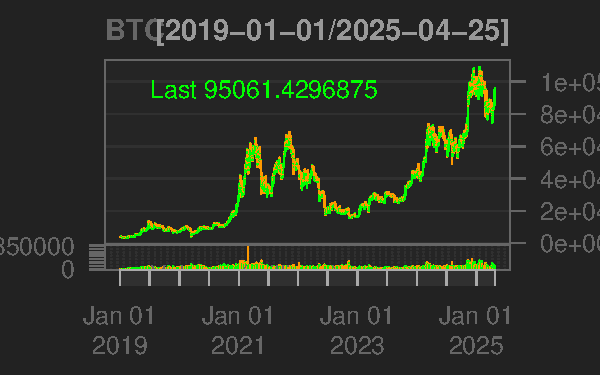
\includegraphics{cripto_update_files/figure-latex/unnamed-chunk-11-1}

\begin{Shaded}
\begin{Highlighting}[]
\FunctionTok{addSMA}\NormalTok{(}\AttributeTok{n =} \DecValTok{50}\NormalTok{, }\AttributeTok{col =} \StringTok{"blue"}\NormalTok{)}
\end{Highlighting}
\end{Shaded}

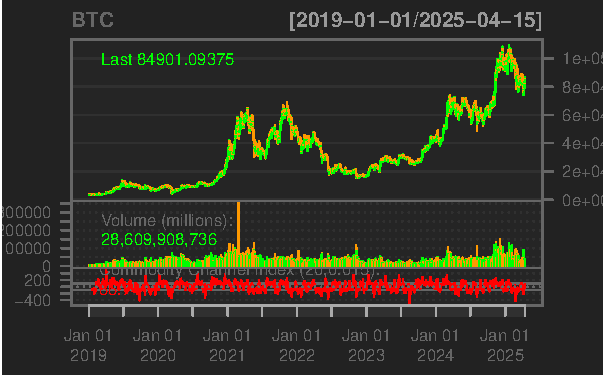
\includegraphics{cripto_update_files/figure-latex/unnamed-chunk-11-2}

\begin{Shaded}
\begin{Highlighting}[]
\FunctionTok{addSMA}\NormalTok{(}\AttributeTok{n =} \DecValTok{100}\NormalTok{, }\AttributeTok{col =} \StringTok{"orange"}\NormalTok{)}
\FunctionTok{legend}\NormalTok{(}\StringTok{"left"}\NormalTok{,}
  \AttributeTok{col =} \FunctionTok{c}\NormalTok{(}\StringTok{"green"}\NormalTok{, }\StringTok{"blue"}\NormalTok{, }\StringTok{"orange"}\NormalTok{),}
  \AttributeTok{legend =} \FunctionTok{c}\NormalTok{(}\StringTok{"SOL{-}USD"}\NormalTok{, }\StringTok{"SMA50"}\NormalTok{, }\StringTok{"SMA100"}\NormalTok{), }\AttributeTok{lty =} \DecValTok{1}\NormalTok{, }\AttributeTok{bty =} \StringTok{"n"}\NormalTok{,}
  \AttributeTok{text.col =} \StringTok{"white"}\NormalTok{, }\AttributeTok{cex =} \FloatTok{0.8}
\NormalTok{)}
\end{Highlighting}
\end{Shaded}

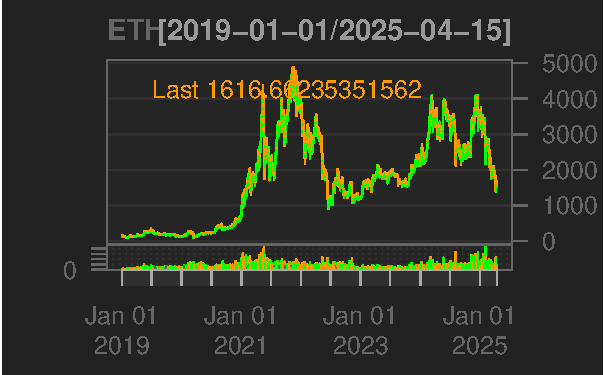
\includegraphics{cripto_update_files/figure-latex/unnamed-chunk-11-3}

\hypertarget{indice-del-canale-delle-materie-prime-cci}{%
\subsubsection{Indice del Canale delle Materie Prime
(CCI):}\label{indice-del-canale-delle-materie-prime-cci}}

Per calcolare il CCI, dobbiamo considerare i prezzi giornalieri di
massimo, minimo e chiusura delle aziende insieme a un periodo di tempo
specificato e un valore costante. In questo passaggio, prenderemo 20
giorni come periodo di tempo e 0,015 come valore costante.

Il seguente codice calcolerà il CCI delle aziende insieme a un grafico:

\begin{Shaded}
\begin{Highlighting}[]
\CommentTok{\# 1.BTC}
\NormalTok{cci\_BTC }\OtherTok{\textless{}{-}} \FunctionTok{CCI}\NormalTok{(}\FunctionTok{HLC}\NormalTok{(BTC), }\AttributeTok{n =} \DecValTok{20}\NormalTok{, }\AttributeTok{c =} \FloatTok{0.015}\NormalTok{)}
\FunctionTok{barChart}\NormalTok{(BTC, }\AttributeTok{theme =} \StringTok{"black"}\NormalTok{)}
\end{Highlighting}
\end{Shaded}

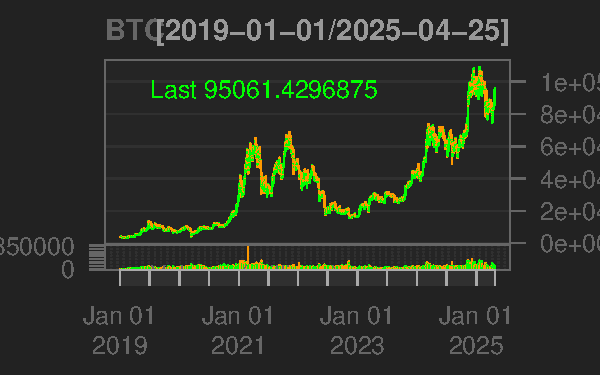
\includegraphics{cripto_update_files/figure-latex/unnamed-chunk-12-1}

\begin{Shaded}
\begin{Highlighting}[]
\FunctionTok{addCCI}\NormalTok{(}\AttributeTok{n =} \DecValTok{20}\NormalTok{, }\AttributeTok{c =} \FloatTok{0.015}\NormalTok{)}
\end{Highlighting}
\end{Shaded}

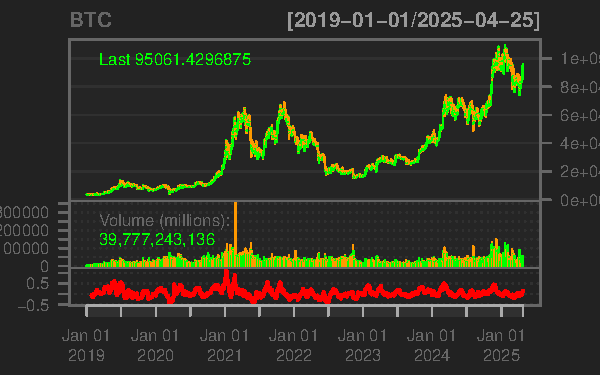
\includegraphics{cripto_update_files/figure-latex/unnamed-chunk-12-2}

\begin{Shaded}
\begin{Highlighting}[]
\CommentTok{\# 2.ETH}
\NormalTok{cci\_eth }\OtherTok{\textless{}{-}} \FunctionTok{CCI}\NormalTok{(}\FunctionTok{HLC}\NormalTok{(ETH), }\AttributeTok{n =} \DecValTok{20}\NormalTok{, }\AttributeTok{c =} \FloatTok{0.015}\NormalTok{)}
\FunctionTok{barChart}\NormalTok{(ETH, }\AttributeTok{theme =} \StringTok{"black"}\NormalTok{)}
\end{Highlighting}
\end{Shaded}

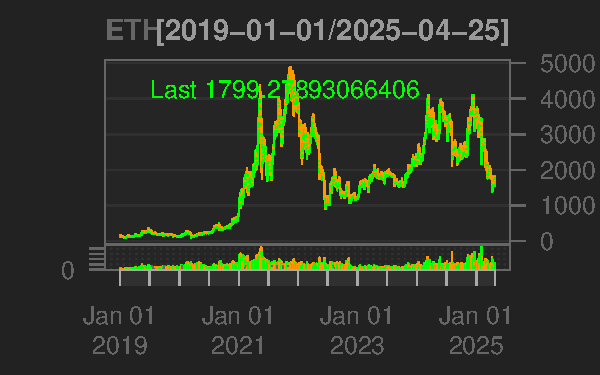
\includegraphics{cripto_update_files/figure-latex/unnamed-chunk-12-3}

\begin{Shaded}
\begin{Highlighting}[]
\FunctionTok{addCCI}\NormalTok{(}\AttributeTok{n =} \DecValTok{20}\NormalTok{, }\AttributeTok{c =} \FloatTok{0.015}\NormalTok{)}
\end{Highlighting}
\end{Shaded}

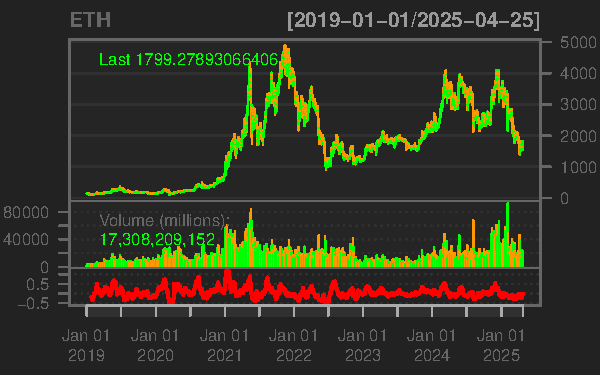
\includegraphics{cripto_update_files/figure-latex/unnamed-chunk-12-4}

\begin{Shaded}
\begin{Highlighting}[]
\CommentTok{\# 3.BNB}
\NormalTok{cci\_BNB }\OtherTok{\textless{}{-}} \FunctionTok{CCI}\NormalTok{(}\FunctionTok{HLC}\NormalTok{(BNB), }\AttributeTok{n =} \DecValTok{20}\NormalTok{, }\AttributeTok{c =} \FloatTok{0.015}\NormalTok{)}
\FunctionTok{barChart}\NormalTok{(BNB, }\AttributeTok{theme =} \StringTok{"black"}\NormalTok{)}
\end{Highlighting}
\end{Shaded}

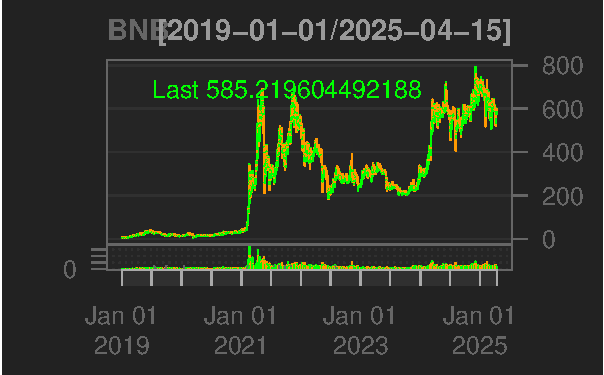
\includegraphics{cripto_update_files/figure-latex/unnamed-chunk-12-5}

\begin{Shaded}
\begin{Highlighting}[]
\FunctionTok{addCCI}\NormalTok{(}\AttributeTok{n =} \DecValTok{20}\NormalTok{, }\AttributeTok{c =} \FloatTok{0.015}\NormalTok{)}
\end{Highlighting}
\end{Shaded}

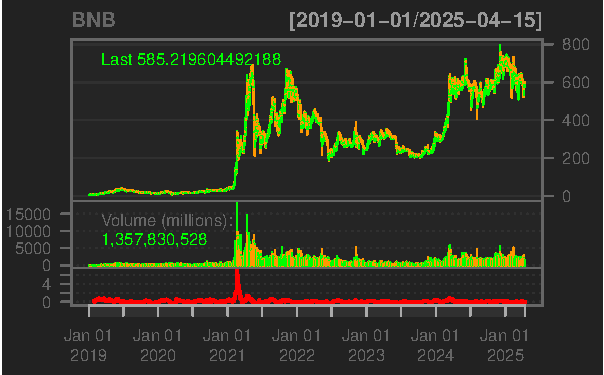
\includegraphics{cripto_update_files/figure-latex/unnamed-chunk-12-6}

\begin{Shaded}
\begin{Highlighting}[]
\CommentTok{\# 4. XRP}

\NormalTok{cci\_XRP }\OtherTok{\textless{}{-}} \FunctionTok{CCI}\NormalTok{(}\FunctionTok{HLC}\NormalTok{(XRP), }\AttributeTok{n =} \DecValTok{20}\NormalTok{, }\AttributeTok{c =} \FloatTok{0.015}\NormalTok{)}
\FunctionTok{barChart}\NormalTok{(XRP, }\AttributeTok{theme =} \StringTok{"black"}\NormalTok{)}
\end{Highlighting}
\end{Shaded}

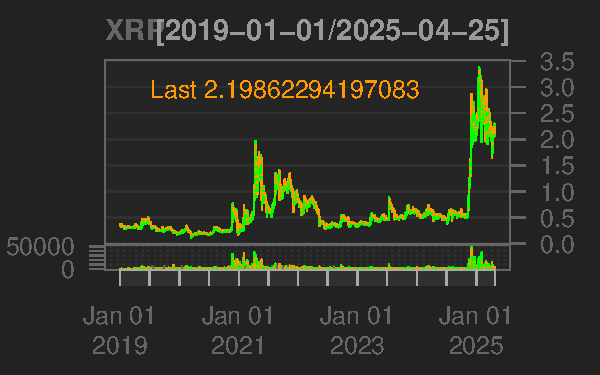
\includegraphics{cripto_update_files/figure-latex/unnamed-chunk-12-7}

\begin{Shaded}
\begin{Highlighting}[]
\FunctionTok{addCCI}\NormalTok{(}\AttributeTok{n =} \DecValTok{20}\NormalTok{, }\AttributeTok{c =} \FloatTok{0.015}\NormalTok{)}
\end{Highlighting}
\end{Shaded}

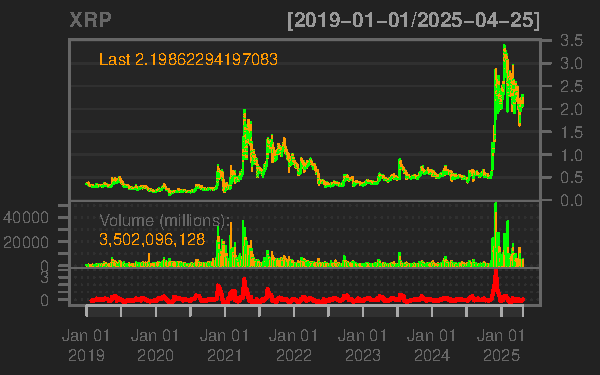
\includegraphics{cripto_update_files/figure-latex/unnamed-chunk-12-8}

\begin{Shaded}
\begin{Highlighting}[]
\CommentTok{\# 5.ADA}

\NormalTok{cci\_ADA }\OtherTok{\textless{}{-}} \FunctionTok{CCI}\NormalTok{(}\FunctionTok{HLC}\NormalTok{(ADA), }\AttributeTok{n =} \DecValTok{20}\NormalTok{, }\AttributeTok{c =} \FloatTok{0.015}\NormalTok{)}
\FunctionTok{barChart}\NormalTok{(ADA, }\AttributeTok{theme =} \StringTok{"black"}\NormalTok{)}
\end{Highlighting}
\end{Shaded}

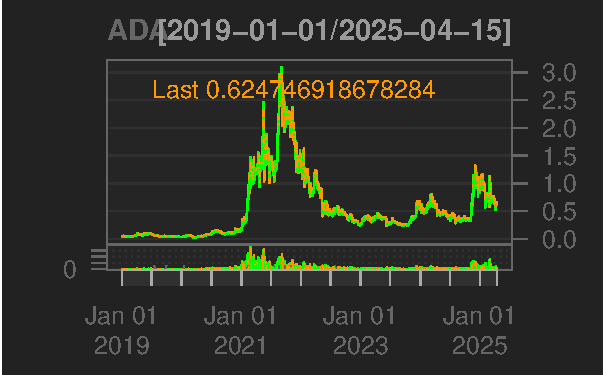
\includegraphics{cripto_update_files/figure-latex/unnamed-chunk-12-9}

\begin{Shaded}
\begin{Highlighting}[]
\FunctionTok{addCCI}\NormalTok{(}\AttributeTok{n =} \DecValTok{20}\NormalTok{, }\AttributeTok{c =} \FloatTok{0.015}\NormalTok{)}
\end{Highlighting}
\end{Shaded}

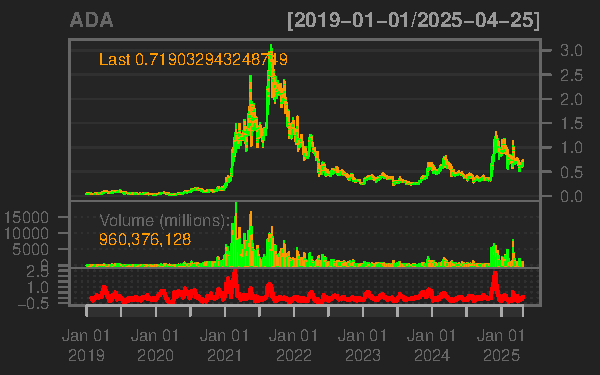
\includegraphics{cripto_update_files/figure-latex/unnamed-chunk-12-10}

\hypertarget{tasso-di-variazione-roc}{%
\subsubsection{Tasso di variazione
(ROC)}\label{tasso-di-variazione-roc}}

Per calcolare il ROC, dobbiamo considerare un intervallo di tempo
specificato e non ci sono restrizioni nell'utilizzare qualsiasi periodo.
In questo passaggio, prenderemo 25 giorni come periodo di tempo.

Il codice seguente calcolerà il ROC delle aziende insieme a un grafico:

\begin{Shaded}
\begin{Highlighting}[]
\CommentTok{\# 1. BTC}
\NormalTok{roc\_btc }\OtherTok{\textless{}{-}} \FunctionTok{ROC}\NormalTok{(BTC}\SpecialCharTok{$}\StringTok{\textasciigrave{}}\AttributeTok{BTC{-}USD.Close}\StringTok{\textasciigrave{}}\NormalTok{, }\AttributeTok{n =} \DecValTok{25}\NormalTok{)}
\FunctionTok{barChart}\NormalTok{(BTC, }\AttributeTok{theme =} \StringTok{"black"}\NormalTok{)}
\end{Highlighting}
\end{Shaded}

\includegraphics{cripto_update_files/figure-latex/unnamed-chunk-13-1}

\begin{Shaded}
\begin{Highlighting}[]
\FunctionTok{addROC}\NormalTok{(}\AttributeTok{n =} \DecValTok{25}\NormalTok{)}
\FunctionTok{legend}\NormalTok{(}\StringTok{"left"}\NormalTok{,}
  \AttributeTok{col =} \StringTok{"red"}\NormalTok{, }\AttributeTok{legend =} \StringTok{"ROC(25)"}\NormalTok{, }\AttributeTok{lty =} \DecValTok{1}\NormalTok{, }\AttributeTok{bty =} \StringTok{"n"}\NormalTok{,}
  \AttributeTok{text.col =} \StringTok{"white"}\NormalTok{, }\AttributeTok{cex =} \FloatTok{0.8}
\NormalTok{)}
\end{Highlighting}
\end{Shaded}

\includegraphics{cripto_update_files/figure-latex/unnamed-chunk-13-2}

\begin{Shaded}
\begin{Highlighting}[]
\NormalTok{roc\_ETH }\OtherTok{\textless{}{-}} \FunctionTok{ROC}\NormalTok{(ETH}\SpecialCharTok{$}\StringTok{\textasciigrave{}}\AttributeTok{ETH{-}USD.Close}\StringTok{\textasciigrave{}}\NormalTok{, }\AttributeTok{n =} \DecValTok{25}\NormalTok{)}
\FunctionTok{barChart}\NormalTok{(ETH, }\AttributeTok{theme =} \StringTok{"black"}\NormalTok{)}
\end{Highlighting}
\end{Shaded}

\includegraphics{cripto_update_files/figure-latex/unnamed-chunk-13-3}

\begin{Shaded}
\begin{Highlighting}[]
\FunctionTok{addROC}\NormalTok{(}\AttributeTok{n =} \DecValTok{25}\NormalTok{)}
\FunctionTok{legend}\NormalTok{(}\StringTok{"left"}\NormalTok{,}
  \AttributeTok{col =} \StringTok{"red"}\NormalTok{, }\AttributeTok{legend =} \StringTok{"ROC(25)"}\NormalTok{, }\AttributeTok{lty =} \DecValTok{1}\NormalTok{, }\AttributeTok{bty =} \StringTok{"n"}\NormalTok{,}
  \AttributeTok{text.col =} \StringTok{"white"}\NormalTok{, }\AttributeTok{cex =} \FloatTok{0.8}
\NormalTok{)}
\end{Highlighting}
\end{Shaded}

\includegraphics{cripto_update_files/figure-latex/unnamed-chunk-13-4}

\begin{Shaded}
\begin{Highlighting}[]
\NormalTok{roc\_BNB }\OtherTok{\textless{}{-}} \FunctionTok{ROC}\NormalTok{(BNB}\SpecialCharTok{$}\StringTok{\textasciigrave{}}\AttributeTok{BNB{-}USD.Close}\StringTok{\textasciigrave{}}\NormalTok{, }\AttributeTok{n =} \DecValTok{25}\NormalTok{)}
\FunctionTok{barChart}\NormalTok{(BNB, }\AttributeTok{theme =} \StringTok{"black"}\NormalTok{)}
\end{Highlighting}
\end{Shaded}

\includegraphics{cripto_update_files/figure-latex/unnamed-chunk-13-5}

\begin{Shaded}
\begin{Highlighting}[]
\FunctionTok{addROC}\NormalTok{(}\AttributeTok{n =} \DecValTok{25}\NormalTok{)}
\FunctionTok{legend}\NormalTok{(}\StringTok{"left"}\NormalTok{,}
  \AttributeTok{col =} \StringTok{"red"}\NormalTok{, }\AttributeTok{legend =} \StringTok{"ROC(25)"}\NormalTok{, }\AttributeTok{lty =} \DecValTok{1}\NormalTok{, }\AttributeTok{bty =} \StringTok{"n"}\NormalTok{,}
  \AttributeTok{text.col =} \StringTok{"white"}\NormalTok{, }\AttributeTok{cex =} \FloatTok{0.8}
\NormalTok{)}
\end{Highlighting}
\end{Shaded}

\includegraphics{cripto_update_files/figure-latex/unnamed-chunk-13-6}

\begin{Shaded}
\begin{Highlighting}[]
\NormalTok{roc\_XRP }\OtherTok{\textless{}{-}} \FunctionTok{ROC}\NormalTok{(XRP}\SpecialCharTok{$}\StringTok{\textasciigrave{}}\AttributeTok{XRP{-}USD.Close}\StringTok{\textasciigrave{}}\NormalTok{, }\AttributeTok{n =} \DecValTok{25}\NormalTok{)}
\FunctionTok{barChart}\NormalTok{(XRP, }\AttributeTok{theme =} \StringTok{"black"}\NormalTok{)}
\end{Highlighting}
\end{Shaded}

\includegraphics{cripto_update_files/figure-latex/unnamed-chunk-13-7}

\begin{Shaded}
\begin{Highlighting}[]
\FunctionTok{addROC}\NormalTok{(}\AttributeTok{n =} \DecValTok{25}\NormalTok{)}
\FunctionTok{legend}\NormalTok{(}\StringTok{"left"}\NormalTok{,}
  \AttributeTok{col =} \StringTok{"red"}\NormalTok{, }\AttributeTok{legend =} \StringTok{"ROC(25)"}\NormalTok{, }\AttributeTok{lty =} \DecValTok{1}\NormalTok{, }\AttributeTok{bty =} \StringTok{"n"}\NormalTok{,}
  \AttributeTok{text.col =} \StringTok{"white"}\NormalTok{, }\AttributeTok{cex =} \FloatTok{0.8}
\NormalTok{)}
\end{Highlighting}
\end{Shaded}

\includegraphics{cripto_update_files/figure-latex/unnamed-chunk-13-8}

\begin{Shaded}
\begin{Highlighting}[]
\NormalTok{roc\_ADA }\OtherTok{\textless{}{-}} \FunctionTok{ROC}\NormalTok{(ADA}\SpecialCharTok{$}\StringTok{\textasciigrave{}}\AttributeTok{ADA{-}USD.Close}\StringTok{\textasciigrave{}}\NormalTok{, }\AttributeTok{n =} \DecValTok{25}\NormalTok{)}
\FunctionTok{barChart}\NormalTok{(ADA, }\AttributeTok{theme =} \StringTok{"black"}\NormalTok{)}
\end{Highlighting}
\end{Shaded}

\includegraphics{cripto_update_files/figure-latex/unnamed-chunk-13-9}

\begin{Shaded}
\begin{Highlighting}[]
\FunctionTok{addROC}\NormalTok{(}\AttributeTok{n =} \DecValTok{25}\NormalTok{)}
\FunctionTok{legend}\NormalTok{(}\StringTok{"left"}\NormalTok{,}
  \AttributeTok{col =} \StringTok{"red"}\NormalTok{, }\AttributeTok{legend =} \StringTok{"ROC(25)"}\NormalTok{, }\AttributeTok{lty =} \DecValTok{1}\NormalTok{, }\AttributeTok{bty =} \StringTok{"n"}\NormalTok{,}
  \AttributeTok{text.col =} \StringTok{"white"}\NormalTok{, }\AttributeTok{cex =} \FloatTok{0.8}
\NormalTok{)}
\end{Highlighting}
\end{Shaded}

\includegraphics{cripto_update_files/figure-latex/unnamed-chunk-13-10}

\begin{Shaded}
\begin{Highlighting}[]
\CommentTok{\# Set the number of successes (3 heads)}
\NormalTok{x }\OtherTok{\textless{}{-}} \DecValTok{3}

\CommentTok{\# Set the number of trials (5 coin flips)}
\NormalTok{size }\OtherTok{\textless{}{-}} \DecValTok{5}

\CommentTok{\# Set the probability of success (0.5 for a fair coin)}
\NormalTok{prob }\OtherTok{\textless{}{-}} \FloatTok{0.5}

\CommentTok{\# Calculate the probability using the dbinom function}
\NormalTok{probability }\OtherTok{\textless{}{-}} \FunctionTok{dbinom}\NormalTok{(x, size, prob)}

\CommentTok{\# Print the result}
\FunctionTok{print}\NormalTok{(probability)}
\end{Highlighting}
\end{Shaded}

\begin{verbatim}
## [1] 0.3125
\end{verbatim}

\hypertarget{generate-random-data-following-a-normal-distribution}{%
\section{Generate random data following a normal
Distribution}\label{generate-random-data-following-a-normal-distribution}}

\begin{Shaded}
\begin{Highlighting}[]
\NormalTok{data }\OtherTok{\textless{}{-}} \FunctionTok{rnorm}\NormalTok{(}\DecValTok{1000}\NormalTok{, }\AttributeTok{mean =} \DecValTok{0}\NormalTok{, }\AttributeTok{sd =} \DecValTok{1}\NormalTok{)}
\CommentTok{\# Plot a histogram of the data}
\FunctionTok{hist}\NormalTok{(data, }\AttributeTok{breaks =} \DecValTok{30}\NormalTok{, }\AttributeTok{col =} \StringTok{"skyblue"}\NormalTok{, }\AttributeTok{main =} \StringTok{"Normal Distribution"}\NormalTok{, }\AttributeTok{xlab =} \StringTok{"Values"}\NormalTok{, }\AttributeTok{ylab =} \StringTok{"Frequency"}\NormalTok{)}
\CommentTok{\# Add a curve representing the probability density function of the normal distribution}
\FunctionTok{curve}\NormalTok{(}\FunctionTok{dnorm}\NormalTok{(x, }\AttributeTok{mean =} \FunctionTok{mean}\NormalTok{(data), }\AttributeTok{sd =} \FunctionTok{sd}\NormalTok{(data)), }\AttributeTok{add =} \ConstantTok{TRUE}\NormalTok{, }\AttributeTok{col =} \StringTok{"red"}\NormalTok{)}
\end{Highlighting}
\end{Shaded}

\includegraphics{cripto_update_files/figure-latex/unnamed-chunk-15-1}

In this example, we first generate a sample of random data following a
normal distribution using the rnorm() function. We then create a
histogram plot of the data using the hist() function, which visualizes
the distribution of the data.

To overlay a curve representing the probability density function of the
normal distribution on the histogram, we use the curve() function with
the dnorm() function to calculate the probability density at each point.

This simple R Markdown code provides a visual and practical
demonstration of the normal distribution, allowing readers to understand
and appreciate this fundamental concept in statistics. ```

\bibliography{skeleton.bib}



\end{document}
